\subsection{1-G, 2-D}

\begin{frame}
\frametitle{One-group, two-dimensional eigenvalue problem}

\begin{columns}
    \column[t]{4cm}
    \begin{itemize}
        \item Problem presented in Brantley and Larsen, 2000 \cite{brantley_simplifiedP3_2000}.
        \item One-energy group.
        \item Two-dimensional problem.
        \item Two materials: fuel and moderator.
    \end{itemize}

    \column[t]{6cm}
    \begin{figure}[htbp!]
        \begin{center}
            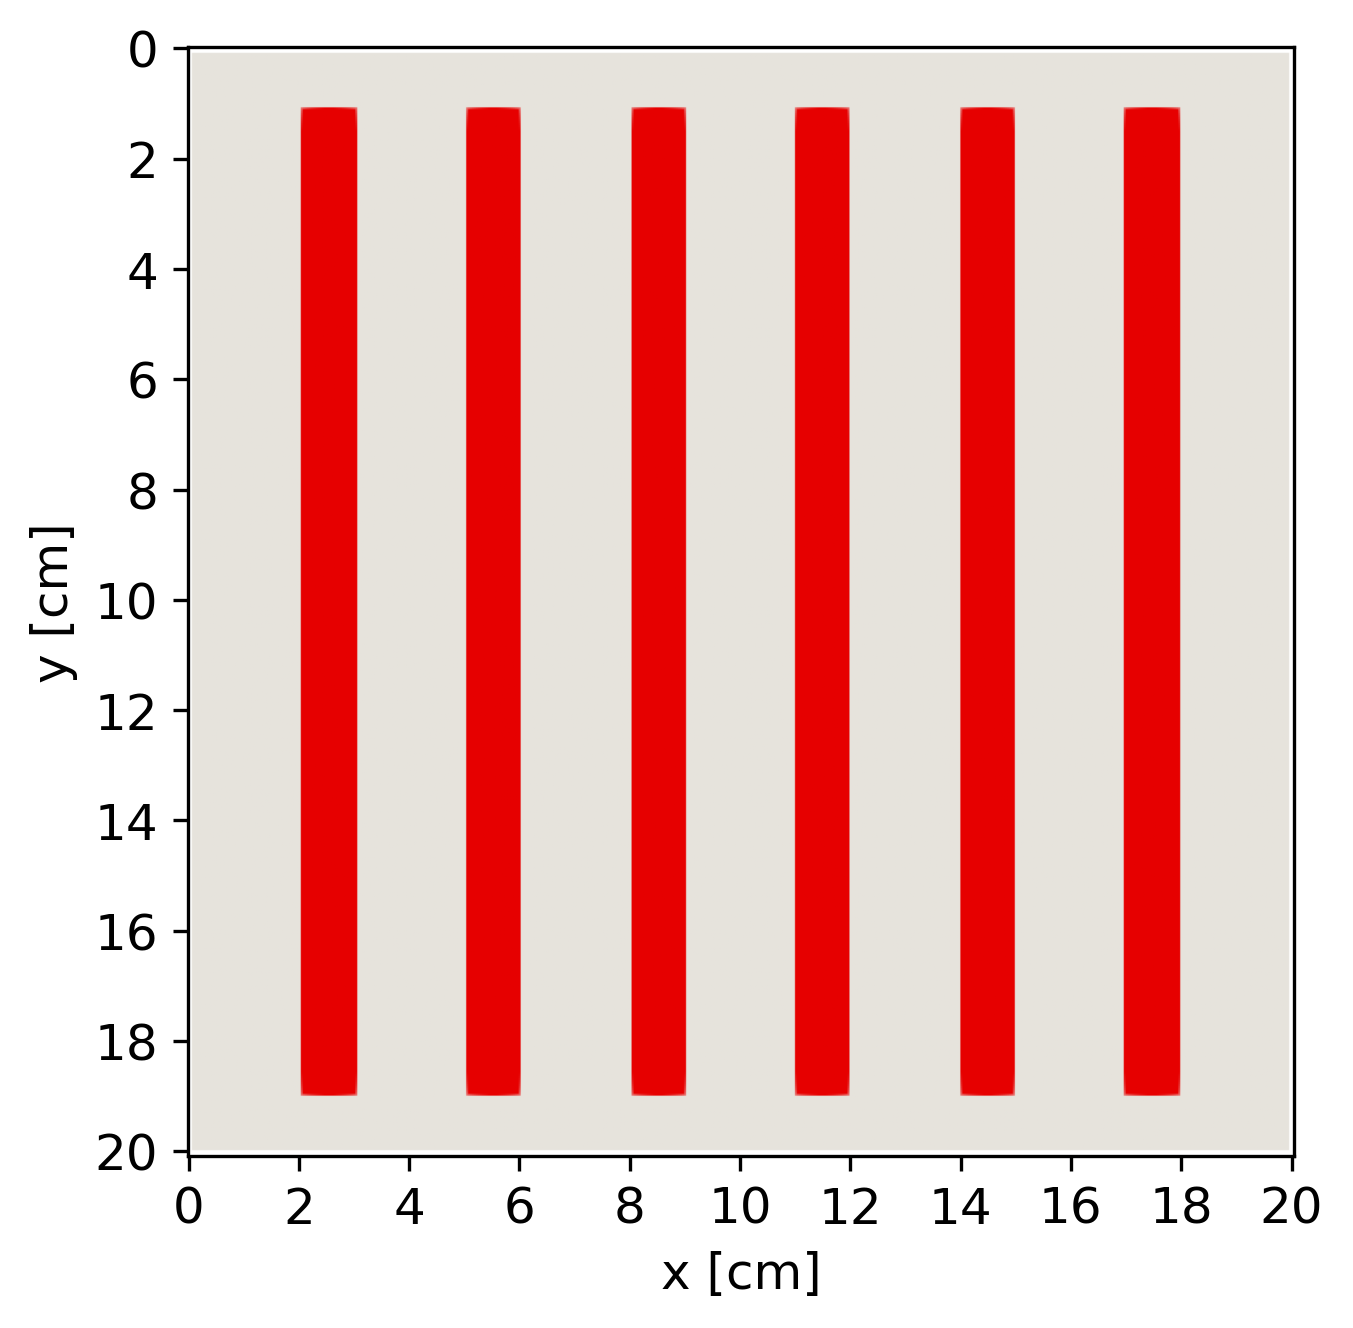
\includegraphics[width=6cm]{figures/mesh2}
        \end{center}
        \caption{Problem's geometry.}
    \end{figure}
\end{columns}
\end{frame}


\begin{frame}
\frametitle{One-group, two-dimensional eigenvalue problem (2)}

    \begin{figure}[htbp!]
        \begin{center}
            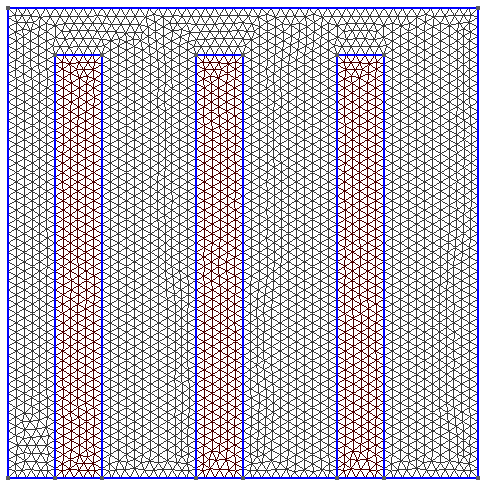
\includegraphics[width=5.5cm]{figures/mesh2b}
        \end{center}
        \caption{Gmsh 2D mesh.}
    \end{figure}
\end{frame}


\begin{frame}
\frametitle{One-group, two-dimensional eigenvalue problem (3)}

\begin{columns}
    \column[t]{4cm}
    \begin{table}[htbp!]
      \centering
      \caption{Eigenvalue comparison.}
      \begin{tabular}{lll}
      \toprule
        $k_{Ref}$ & $k_{SP_3}$  & $\Delta_{\rho}$ \\
      \midrule
        0.79862   & 0.79854     & 12        \\
      \bottomrule
      \end{tabular}
    \end{table}

    \column[t]{6cm}
    \begin{figure}[htbp!]
        \begin{center}
            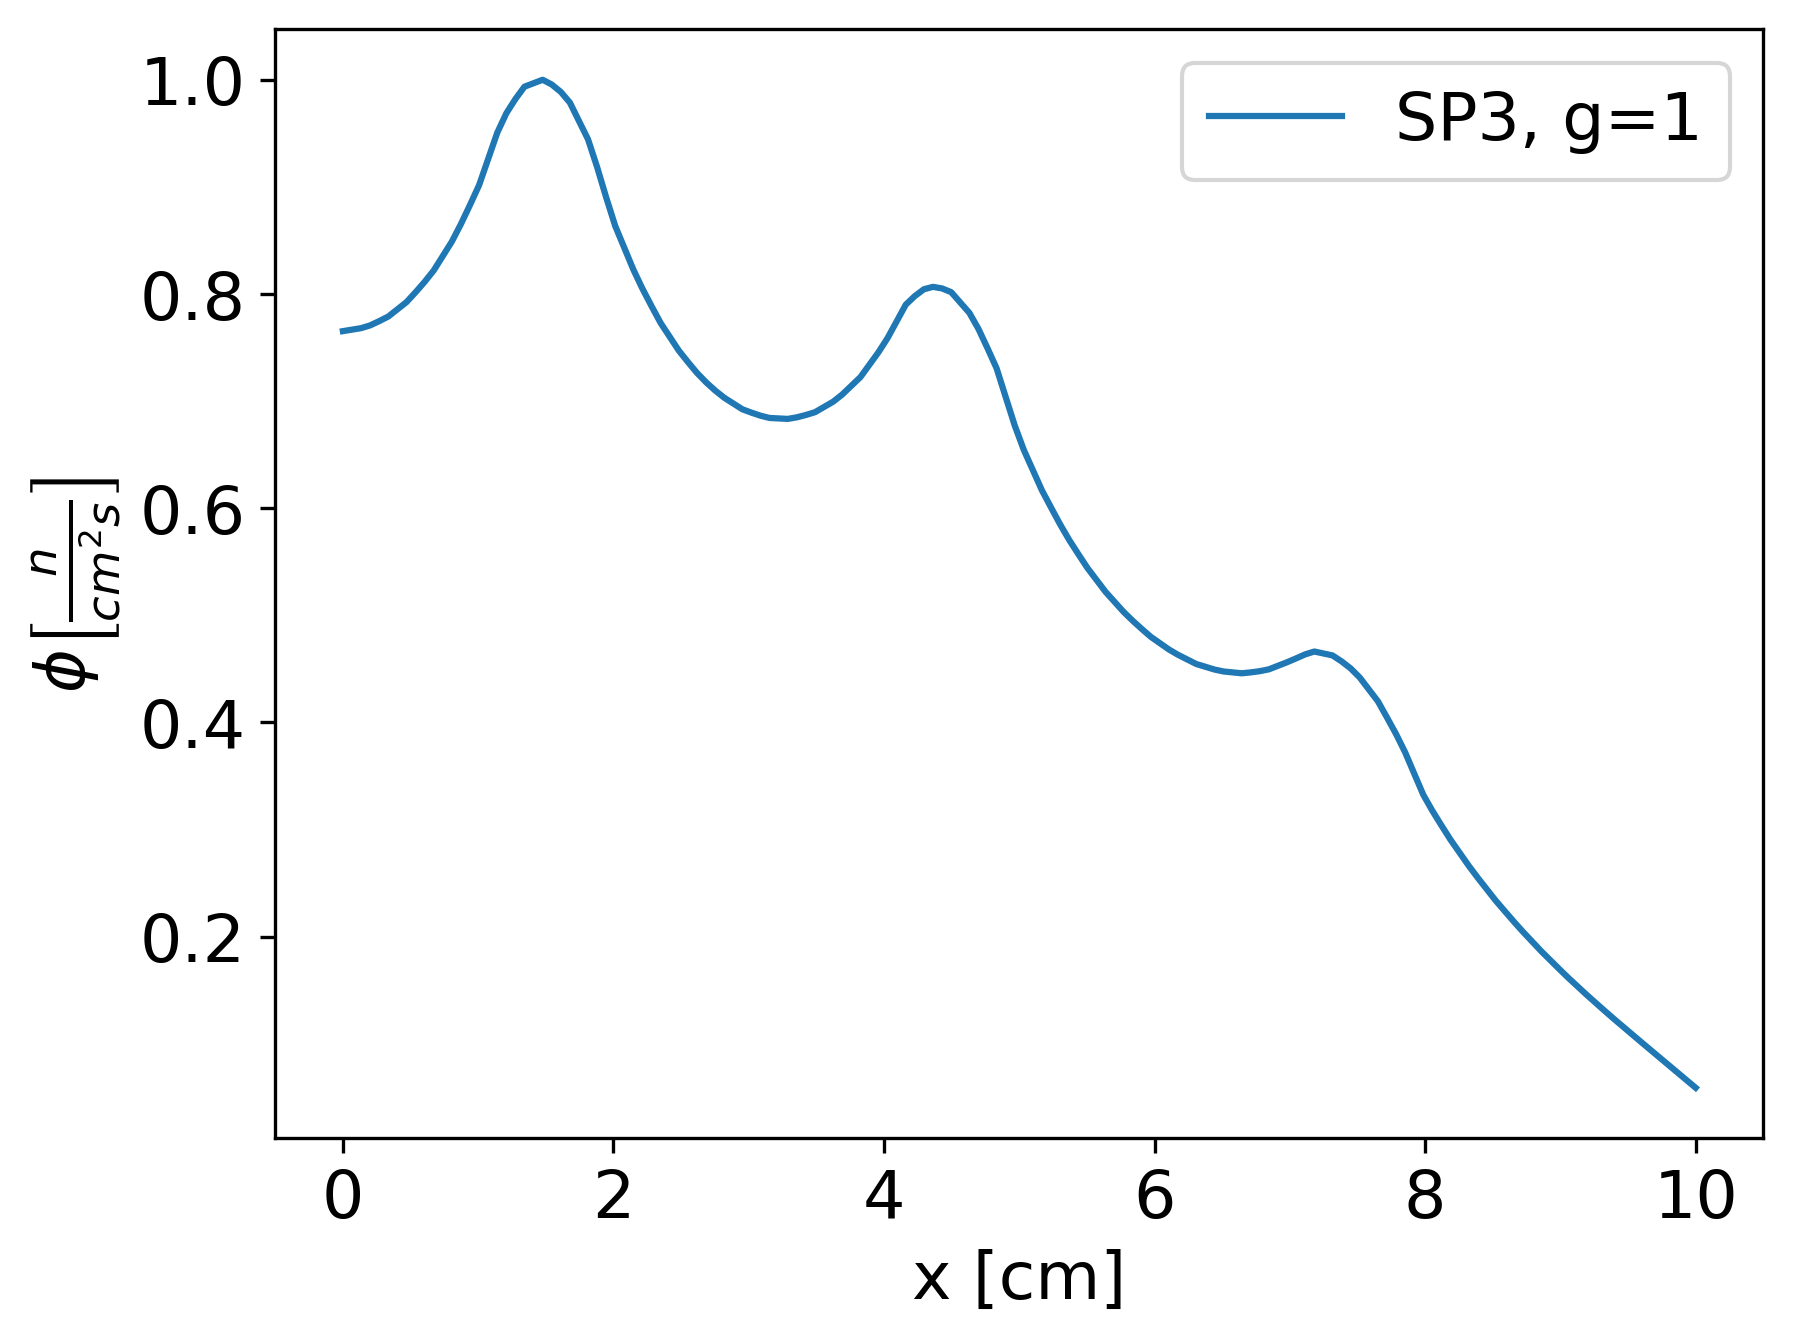
\includegraphics[width=6cm]{figures/flux-output}
        \end{center}
        \caption{Scalar flux over line at y=4.5 cm.}
    \end{figure}
\end{columns}
\end{frame}


\subsection{2-G, 2-D}

\begin{frame}
\frametitle{C5 MOX Benchmark}

    \begin{itemize}
        \item Exercise defined in 1994 by OECD/NEA \cite{cavarec_benchmark_1994}.
        \item Two-energy groups.
        \item Two-dimensional problem.
        \item Two types of fuel: UO$_2$, MOX.
    \end{itemize}
\end{frame}


\begin{frame}
\frametitle{C5 MOX Benchmark (2)}

\begin{columns}
    \column[t]{5cm}
    \begin{figure}[htbp!]
        \begin{center}
            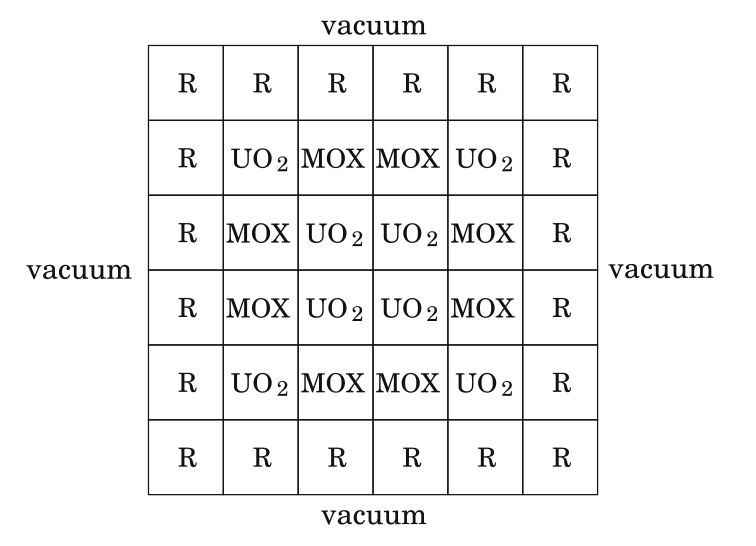
\includegraphics[width=5cm]{figures/bench-config}
        \end{center}
        \caption{2-D C5 MOX benchmark configuration. $R$ represents the reflectors. Image reproduced from \cite{capilla_applications_2009}.}
    \end{figure}

    \column[t]{6cm}
    \begin{figure}[htbp!]
        \begin{center}
            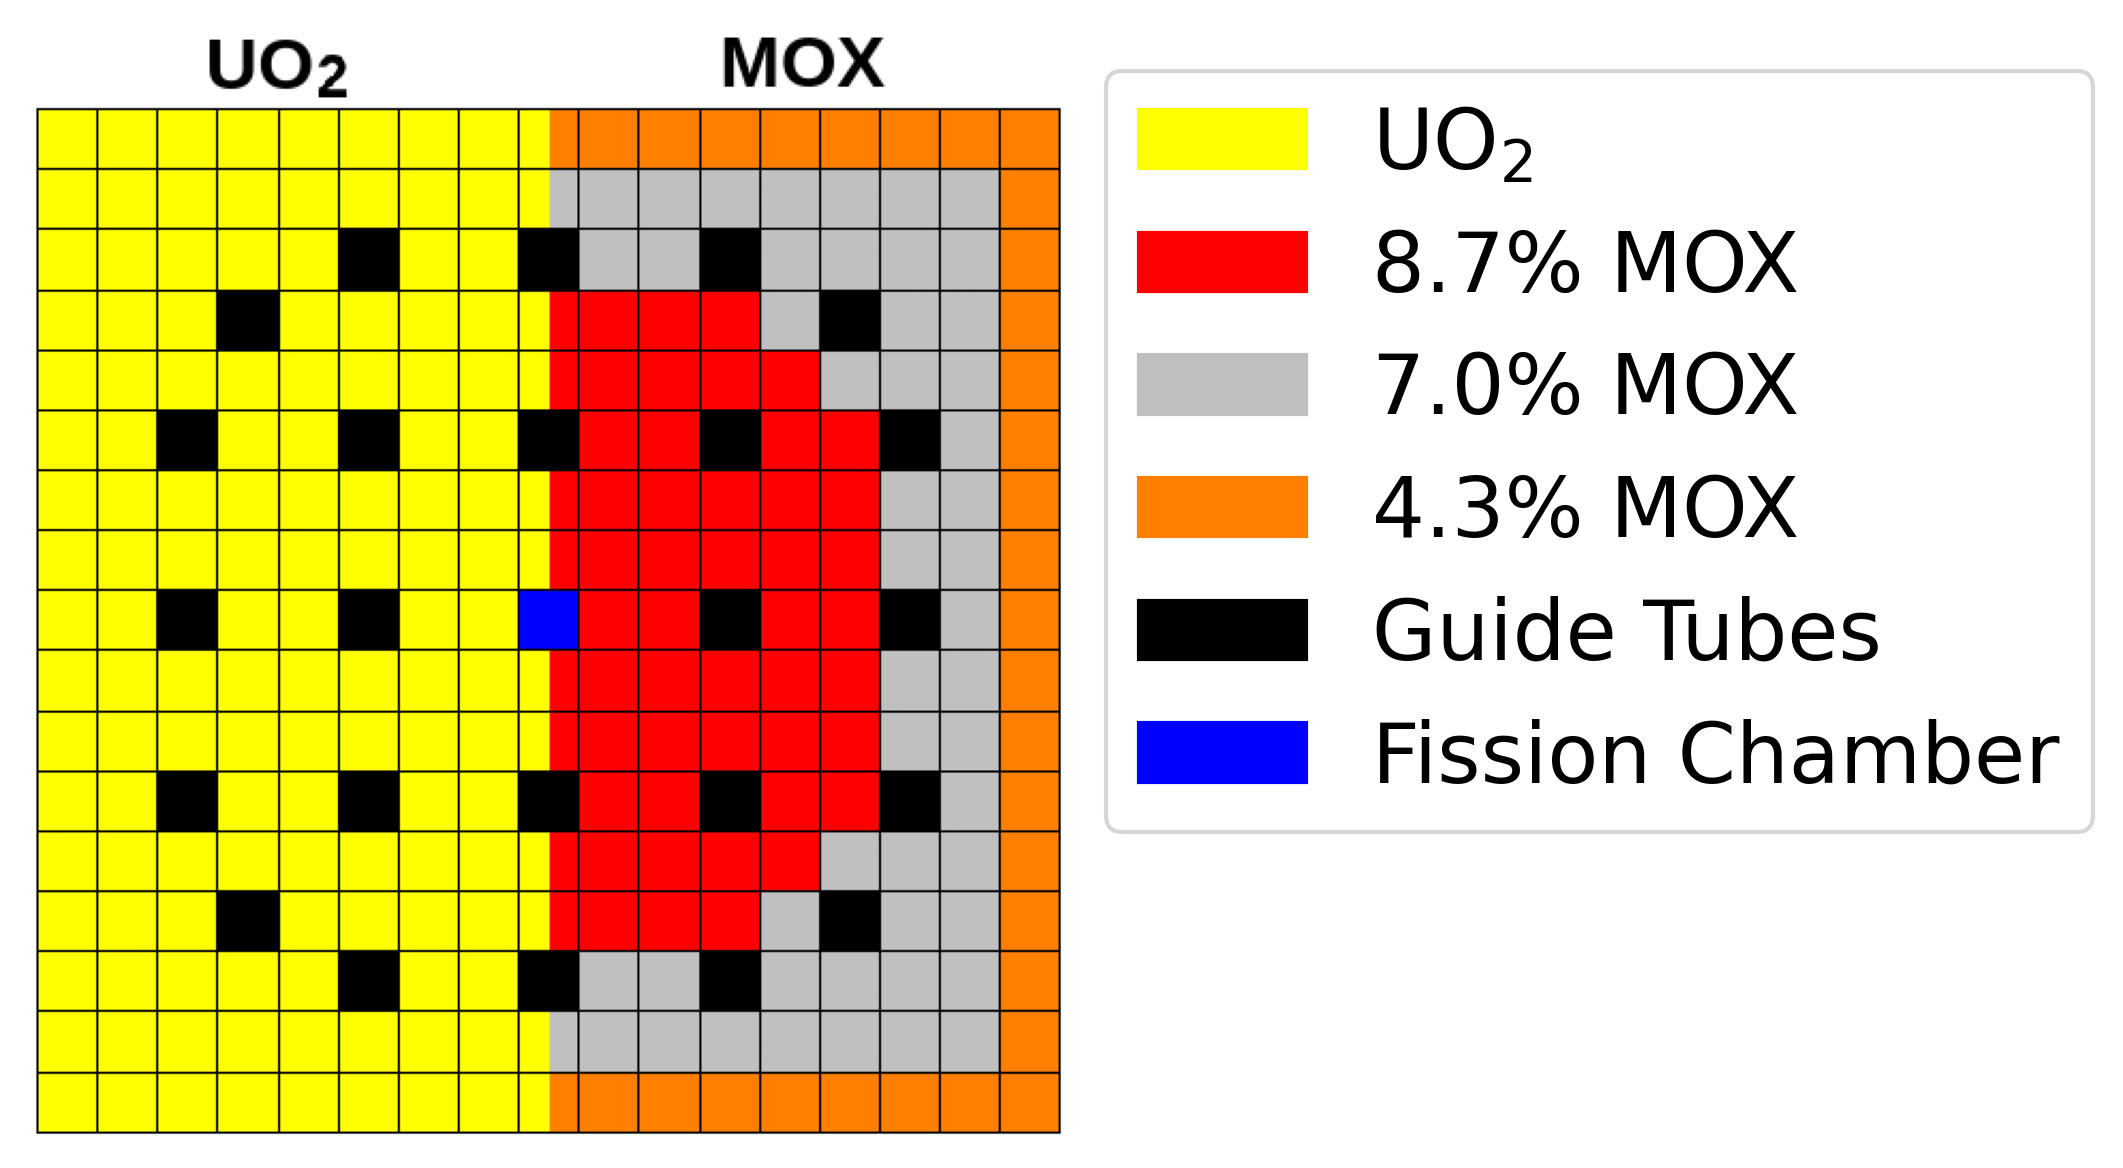
\includegraphics[width=6cm]{figures/bench-config2B}
        \end{center}
        \caption{Structure of the UO2 and MOX assemblies.}
    \end{figure}
\end{columns}
\end{frame}


\begin{frame}
\frametitle{C5 MOX Benchmark (3)}

    \begin{figure}[htbp!]
        \begin{center}
            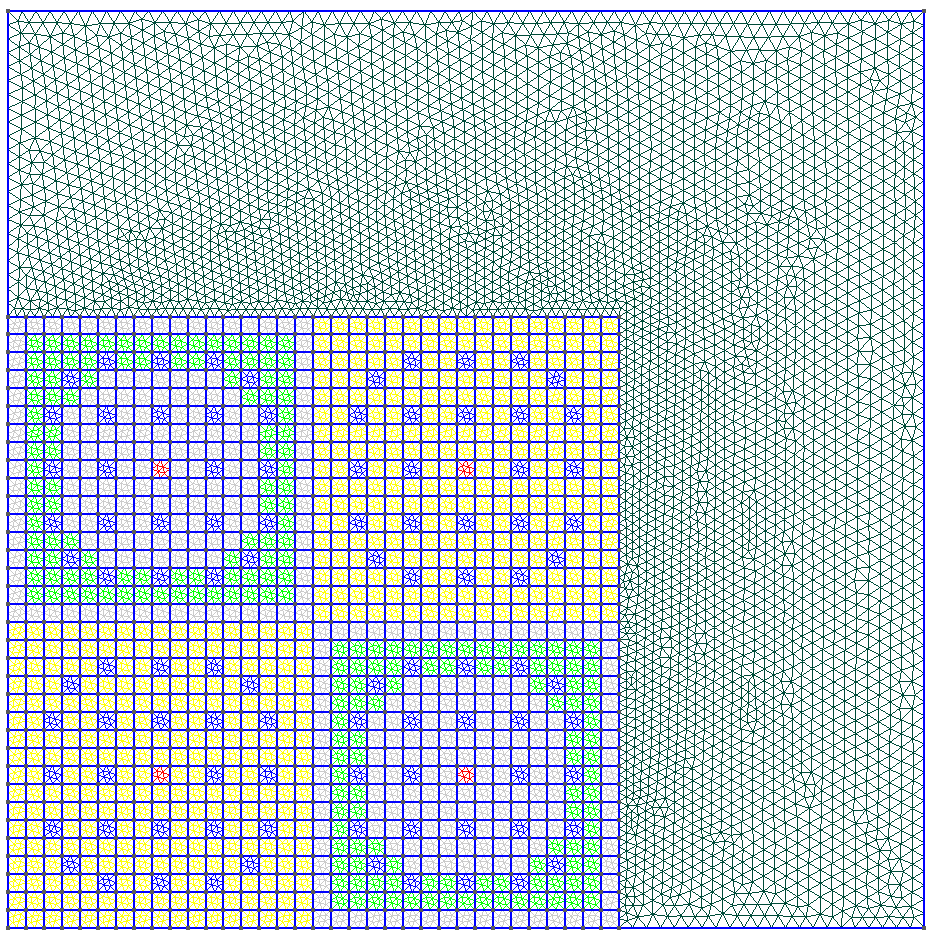
\includegraphics[width=6.cm]{figures/bench-mesh}
        \end{center}
        \caption{Gmsh 2D mesh.}
    \end{figure}

\end{frame}

\begin{frame}
\frametitle{C5 MOX Benchmark (4)}

% Clarification on the cross-sections

If the higher order information of the scattering cross-section is not available (no correction):
\begin{align}
  & D_{0,g} = \frac{1}{3 \Sigma_{1,g}} = \frac{1}{3 \Sigma_{t,g}}
\end{align}

The definition of the benchmark \cite{cavarec_benchmark_1994} recommends applying the diagonal transport correction:
\begin{align}
  & D_{0,g} = \frac{1}{3 \Sigma_{tr,g}} \label{eq:diff-tr} \\
  & \Sigma_{tr, g} = \Sigma_{t,g} - \bar{\mu}_{g} \Sigma_{s0,g} \notag
  \intertext{where}
  & \Sigma_{tr, g} = \mbox{group $g$ transport cross-section} \notag \\
  & \bar{\mu}_{g} = \mbox{group $g$ average cosine deviation angle.} \notag
\end{align}

\end{frame}


\begin{frame}
\frametitle{C5 MOX Benchmark (5)}
	\begin{table}[htbp!]
	\centering
	\begin{tabular}{lccc}
	\toprule
	 & C5G2 Benchmark      & \multicolumn{2}{c}{Cerberus}          \\
	\midrule
	Case & $k_{Ref}$       & $k_{SP_3}$ & $\Delta_\rho$ [pcm] \\
	\midrule
	No correction          & 0.96969  & 0.97106  & 145  \\
	Transport correction   & 0.93755  & 0.93792  &  43  \\
	\bottomrule
	\end{tabular}
	\label{tab:2d-keff}
	\end{table}
\end{frame}


\begin{frame}
\frametitle{C5 MOX Benchmark (6)}

\begin{columns}
    \column[t]{5.5cm}
    \begin{figure}[htbp!]
        \begin{center}
            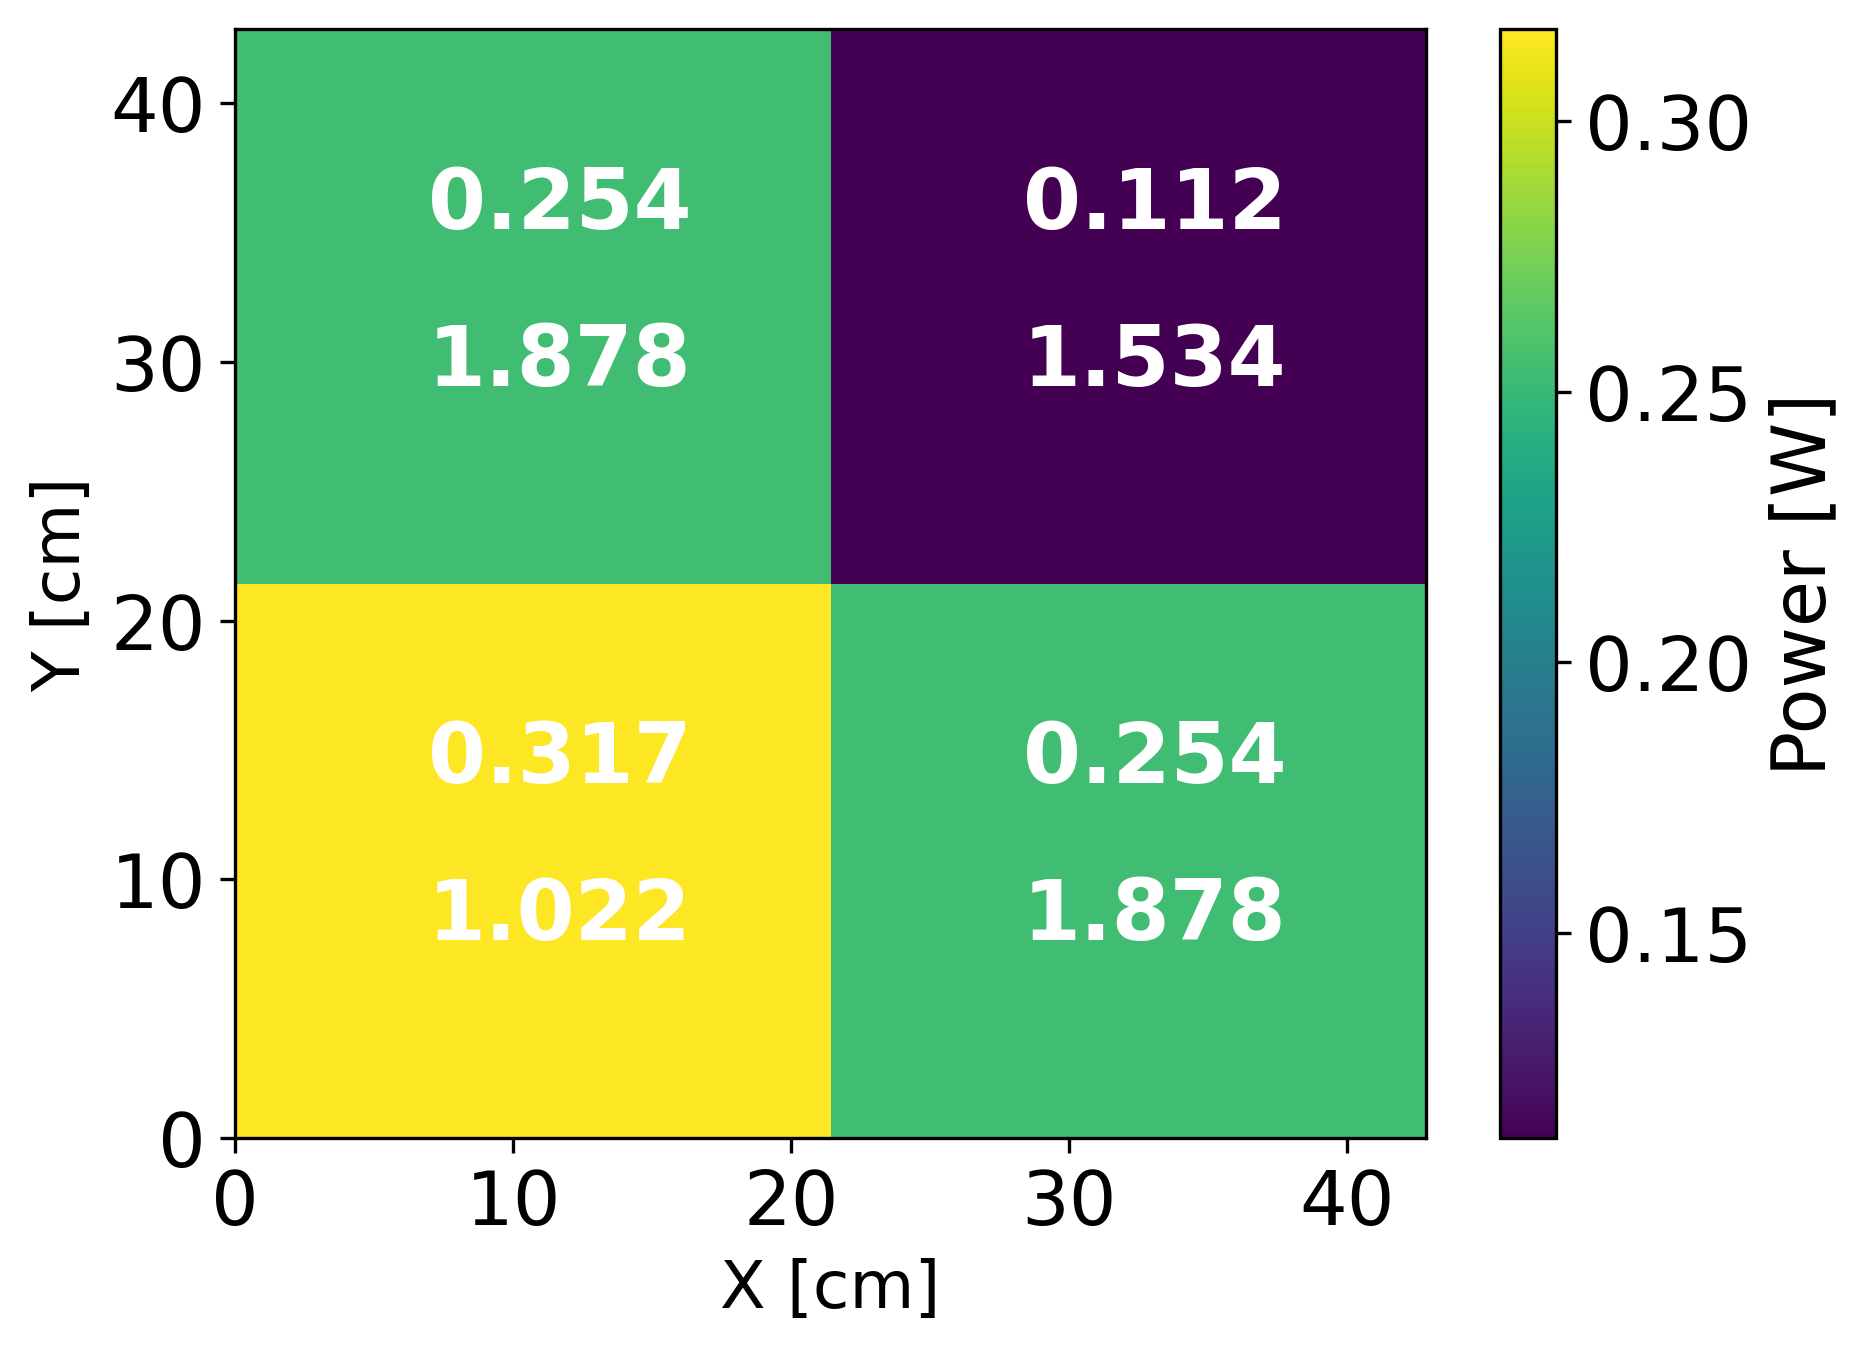
\includegraphics[width=6.cm]{figures/distrib}
        \end{center}
        \caption{Assembly power distribution. Top: Assembly power. Bottom: Pin power relative difference expressed in \%.}
    \end{figure}

    \column[t]{5.5cm}
    \begin{figure}[htbp!]
        \begin{center}
            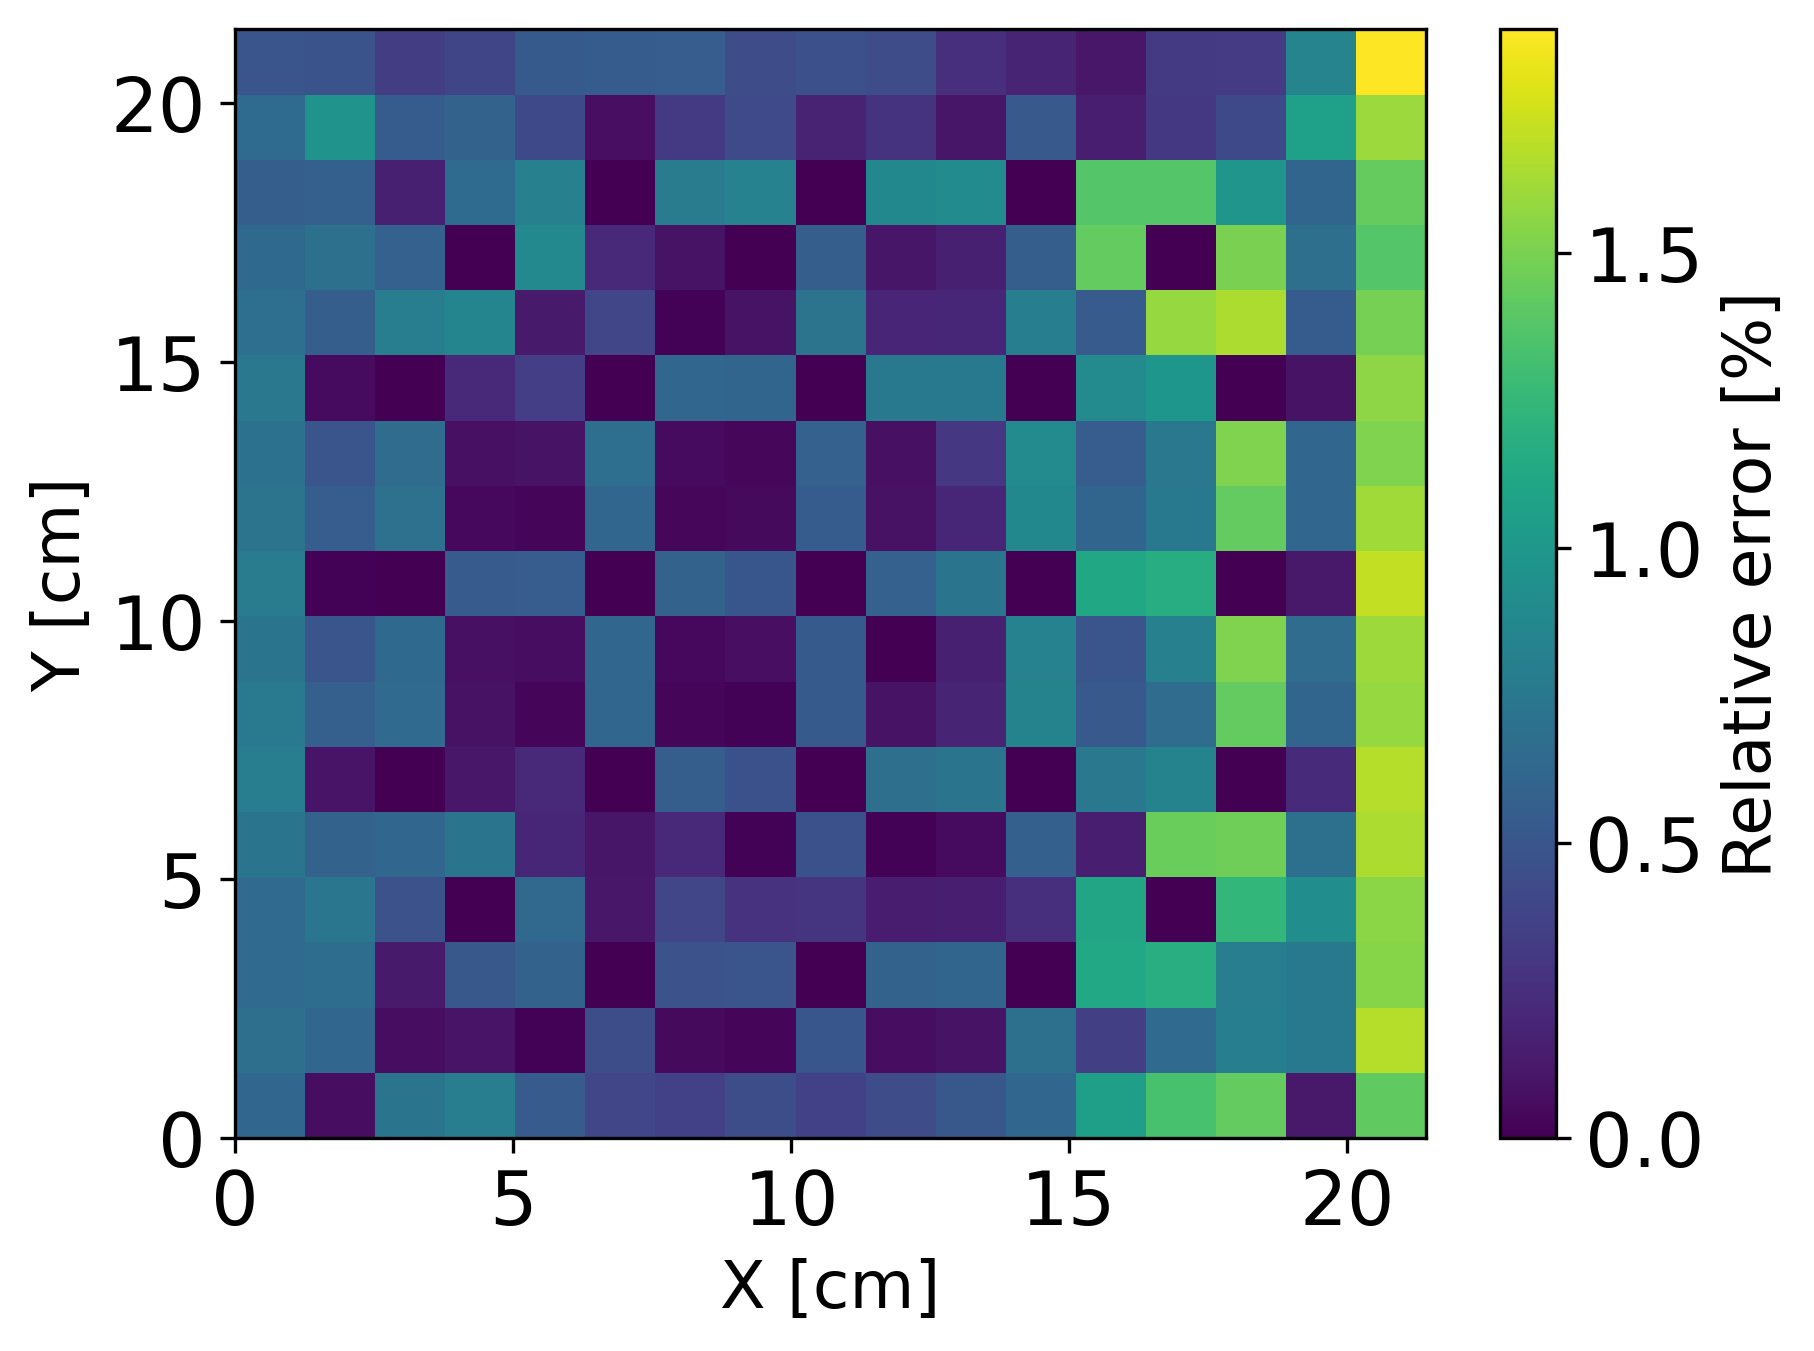
\includegraphics[width=6.cm]{figures/mox-r-pin-by-pin}
        \end{center}
        \caption{MOX assembly pin power relative difference expressed in \%.}
    \end{figure}

\end{columns}
\end{frame}


\begin{frame}
\frametitle{C5 MOX Benchmark (7)}

    \begin{figure}[htbp!]
        \begin{center}
            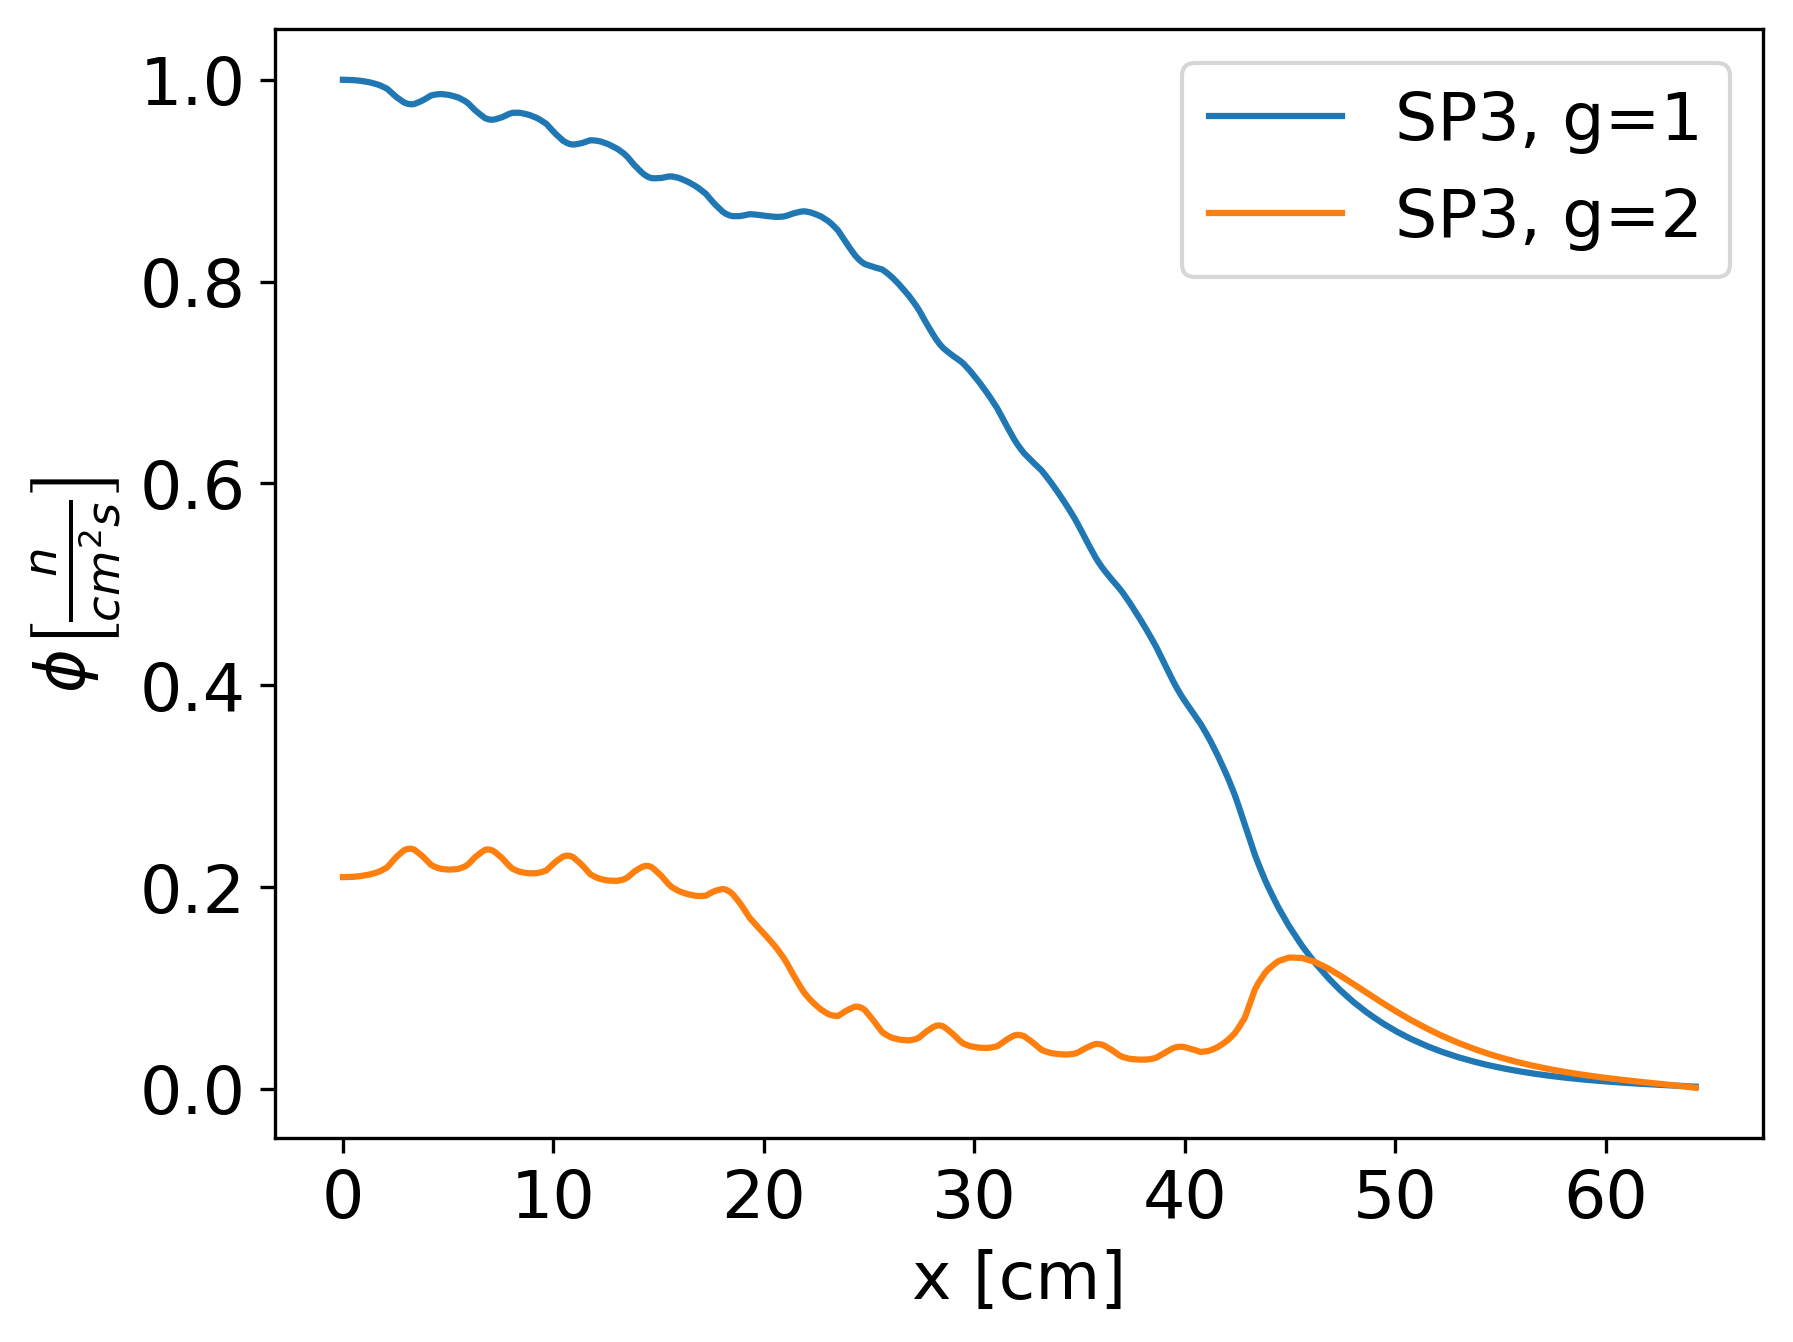
\includegraphics[width=6cm]{figures/sp3-flux-output-correct}
        \end{center}
        \caption{Scalar flux at y=10.71cm.}
    \end{figure}

\end{frame}


\subsection{2-G, 3-D}

\begin{frame}
\frametitle{C5 MOX 3D}

\begin{columns}
    \column[t]{4cm}
    \begin{itemize}
        \item 3D mini-core variation of the C5 MOX benchmark introduced by Ryu et al., 2013 \cite{ryu_finite_2013}.
        \item Two-energy group.
        \item Three-dimensional problem.
        \item Three materials: fuel, moderator, and reflector.
    \end{itemize}

    \column[t]{6cm}
    \begin{figure}[htbp!]
        \begin{center}
            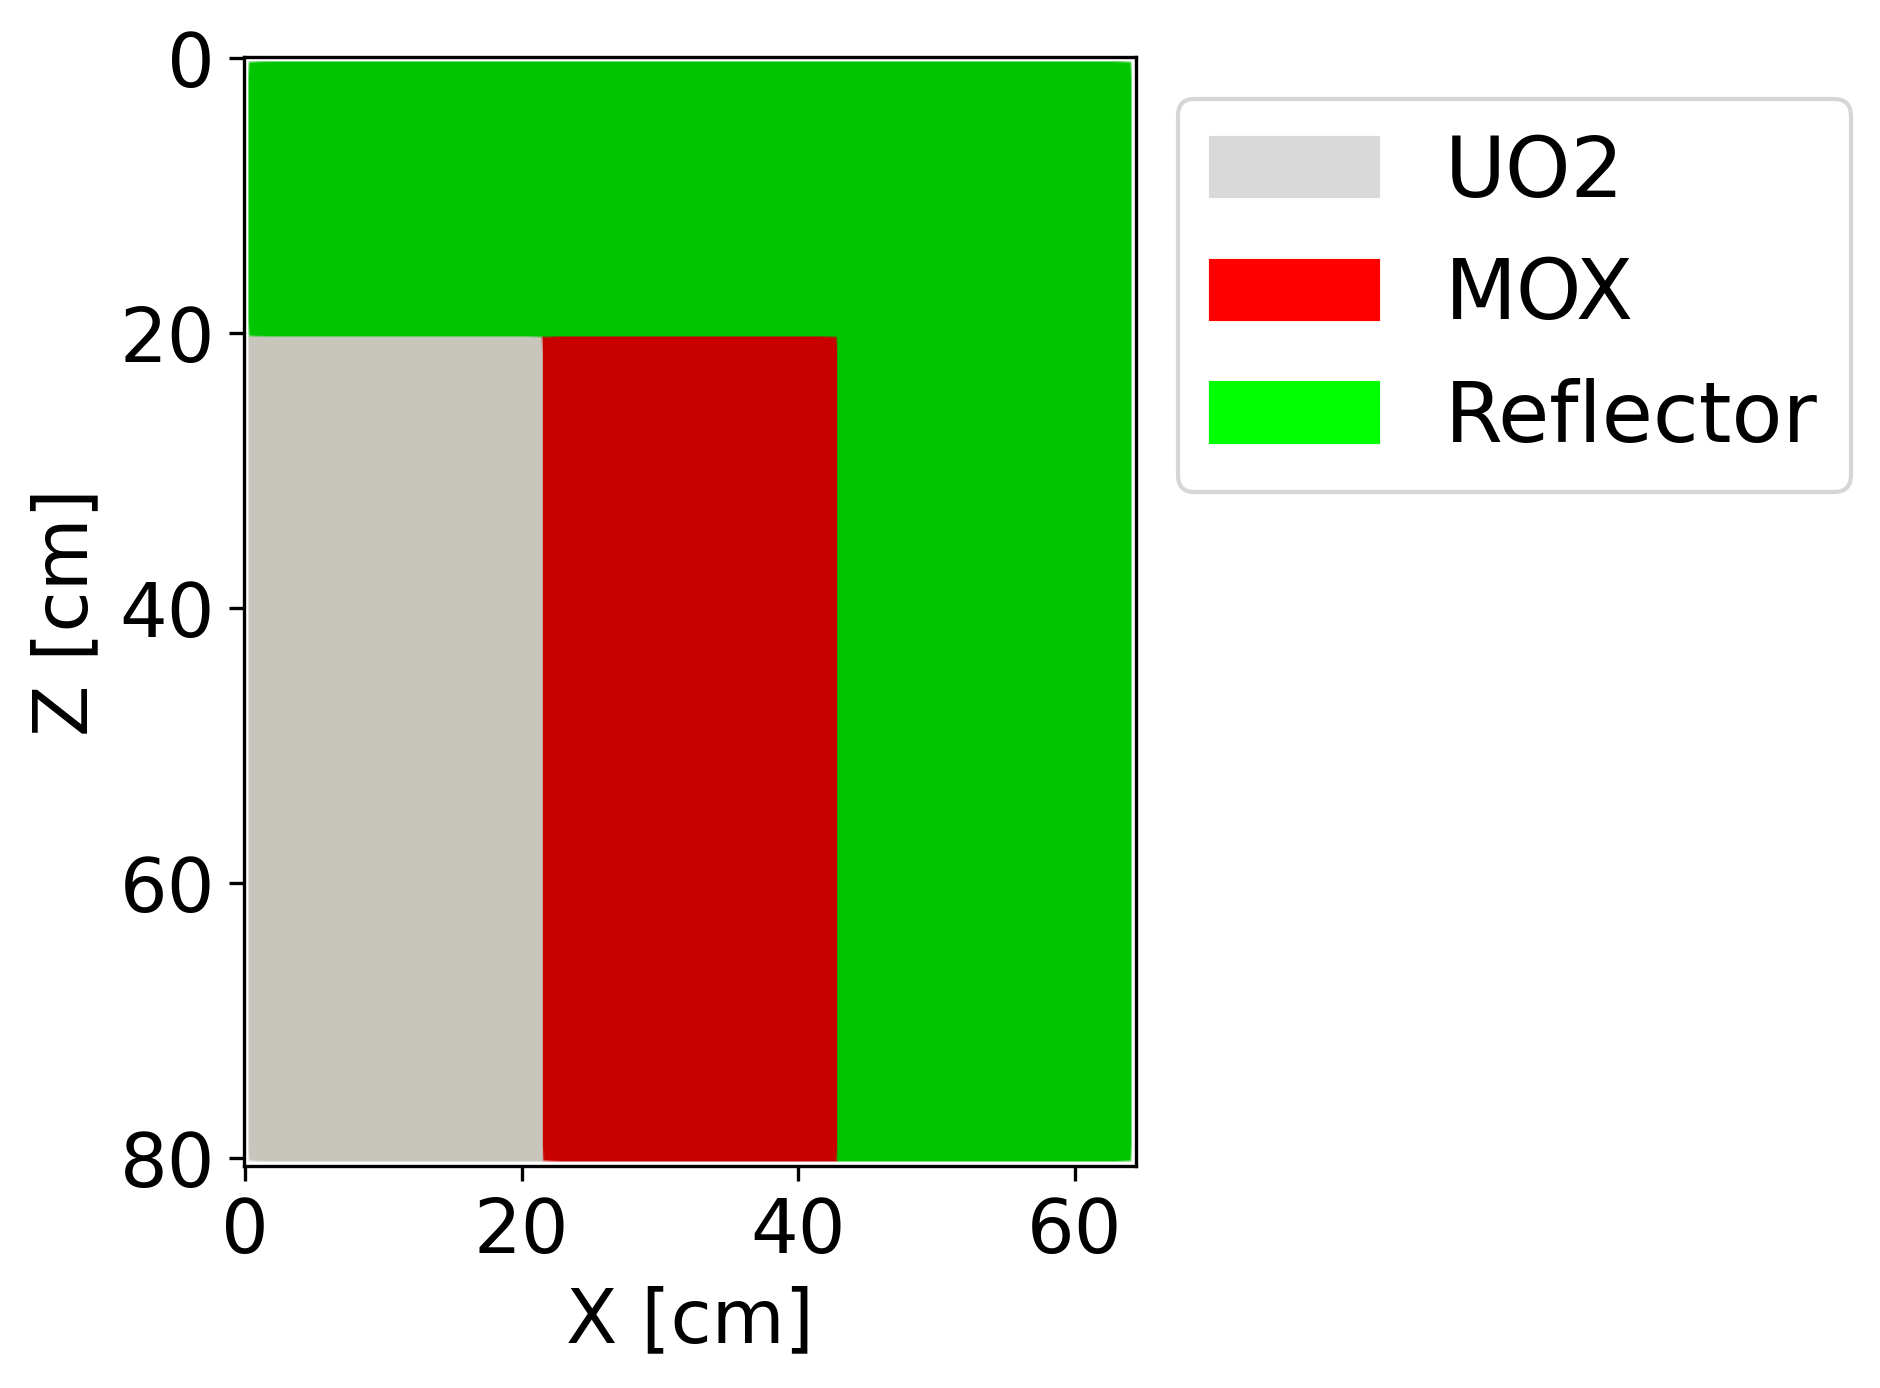
\includegraphics[width=6cm]{figures/geo-xz2}
        \end{center}
        \caption{Axial layout of the C5G2 3D Benchmark.}
    \end{figure}
\end{columns}
\end{frame}


\begin{frame}
\frametitle{C5 MOX 3D (2)}

\begin{columns}
    \column[t]{4cm}
    \begin{table}[htbp!]
      \centering
      \caption{Eigenvalue comparison.}
      \begin{tabular}{lll}
      \toprule
        $k_{Ref}$ & $k_{SP_3}$  & $\Delta_{\rho}$ \\
      \midrule
        0.91974   & 0.91979     & 6               \\
      \bottomrule
      \end{tabular}
    \end{table}

    \column[t]{6cm}
    \begin{figure}[htbp!]
        \begin{center}
            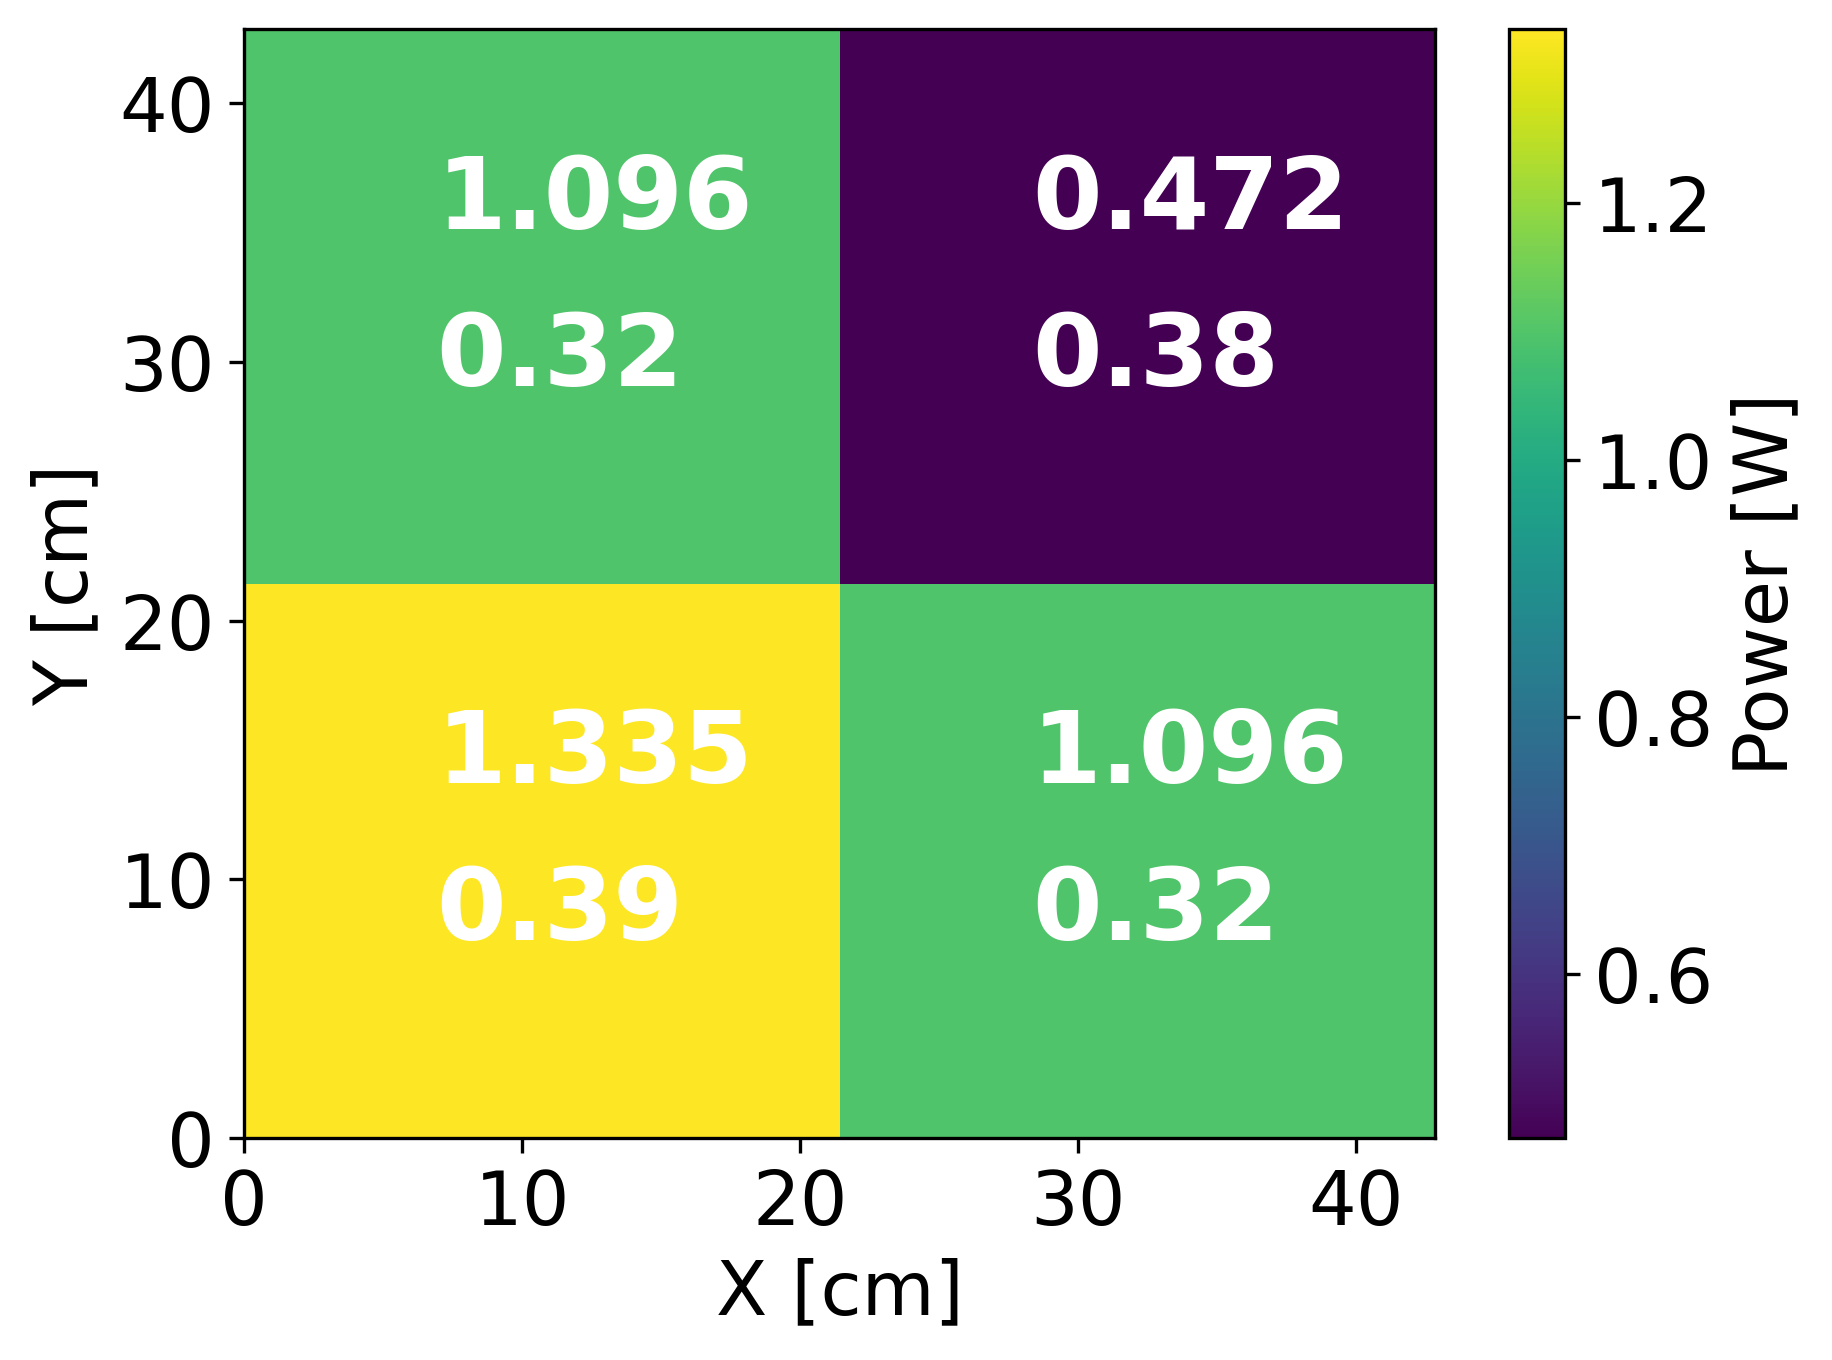
\includegraphics[width=6cm]{figures/C5G23D-distrib}
        \end{center}
        \caption{Power distribution in the C5G2 3D Benchmark. Top: power distribution. Bottom: relative difference expressed in \%.}
    \end{figure}
\end{columns}
\end{frame}
